\documentclass[portuguese,oneside]{tcc}

\usepackage{graphicx}
\usepackage{multirow}
\usepackage{nicefrac}
\usepackage{algorithmic}
\usepackage{calc}
\usepackage{enumitem}
\usepackage{fixltx2e}

\author{Guilherme de Mello Mattos Taschetto e Pedro Pillon Vanzella}

\title{Inteligência Artificial Aplicada a Elevadores}
      {Artificial Intelligence Applied to Elevators}

\tipotrabalho{\ptci}
\curso{\cc}
\orientador{João Batista de Oliveira}

\begin{document}

\begin{resumo}{elevadores, inteligência artificial, simulação, sistemas multiagentes, aprendizado de máquina}
Elevadores são um meio de transporte utilizados por milhões de pessoas no mundo
inteiro. Com este trabalho, pretende-se propor soluções de Inteligência
Artificial para melhorar a eficiência dos mesmos, reduzindo o tempo o qual
passageiros despendem em função destes. Através da modelagem e de implementações
de um simulador de elevadores e de algoritmos de Inteligência Artificial,
espera-se realizar testes de diferentes técnicas e soluções propostas na
literatura, a fim de propor quais estratégias são mais adequadas para cada
cenário.
\end{resumo}

\begin{abstract}{elevators, artificial inteligence, simulation, multiagent systems, machine learning}
  Elevators are a mode of transportation used by milions of people around the
  world. In this project, we will propose Artificial Inteligence solutions in
  order to increase their efficiency, reducing their users' wait times.
  A simulator must be built in order to test the different solutions proposed in
  the existing literature, as well as a few new solutions.
\end{abstract}

\tableofcontents

\chapter{\label{chap:intro}Introdução}

Em 2014, 54\% da população mundial vivia em áreas urbanas, de acordo com a Organização das Nações Unidas \cite{UN14}. A expectativa é que esta proporção aumente para 66\% até o ano 2050. Em números absolutos isto representa um acréscimo de 2,5 bilhões de pessoas à população urbana mundial nos próximos 35 anos. Uma das consequências da alta densidade populacional em regiões geográficas limitadas é o crescimento do modelo de verticalização na construção civil. Neste cenário, onde prédios de diversos andares se tornam presença no cotidiano da maioria da população, os elevadores passam a um papel de destaque.

Uma pesquisa realizada pela IBM no ano de 2010 em 16 cidades norte-americanas constatou que, durante 12 meses, o tempo acumulado no qual trabalhadores de escritórios\footnote{Em uma força de trabalho total de 51 milhões de trabalhadores, dos quais 12,7 milhões são usuários de elevadores diariamente \cite{IBM10}.} aguardaram por elevadores foi de 92 anos \cite{IBM10}. Em uma economia onde o salário horário médio de um trabalhador é de US\$ 24,99, o tempo de espera por elevadores representa custos de mais de US\$ 20 bilhões em média por ano \cite{BLS15}.

Além do impacto econômico existe o impacto psicológico. Trabalhadores em centros metropolitanos empreendem uma parcela significativa da sua rotina no deslocamento entre residência e local de trabalho e no caminho inverso ao final do dia. Além de gastar uma quantidade significativa de tempo no trânsito das ruas, em carros, ônibus, bicicletas e metrôs, o tempo compreendido entre aguardar o elevador e desembarcar no andar desejado está longe de ser desprezível. Em função disso, ajustam sua rotina abrindo mão de momentos de momentos de descanso ou lazer. Uma possível consequência é um aumento nos níveis de estresse e um decréscimo na qualidade de vida a médio e longo prazo. {\color{red}[BUSCAR FONTES PARA ESTE PARÁGRAFO]} % TODO: CITATIONNEEDED

\begin{figure}[htb!]
\centering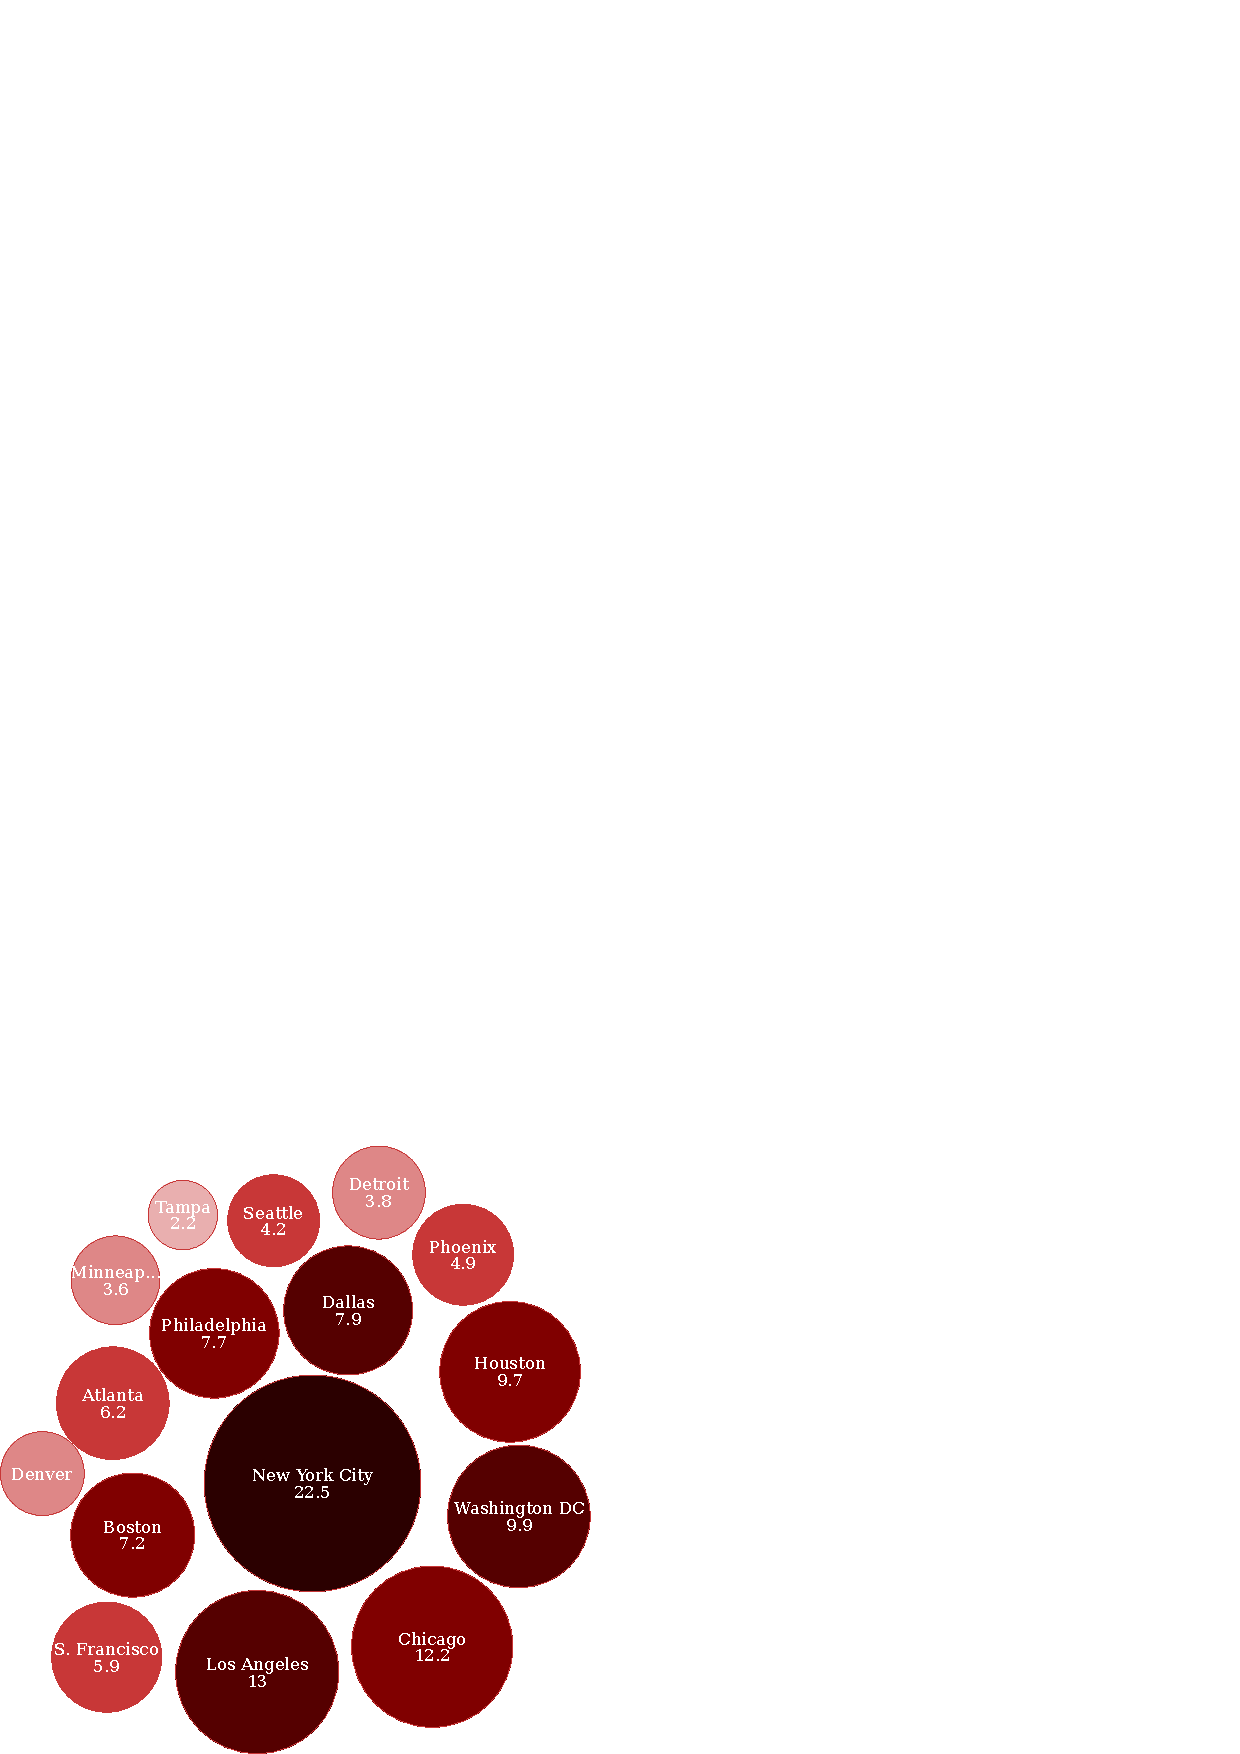
\includegraphics{img/time-cost.jpg}
\caption{\label{fig:fig1}Tempo de espera acumulado (em anos) por elevadores durante 12 meses em 16 cidades norte-americanas. Fonte: \cite{IBM10}}
\end{figure}

Neste contexto global, a indústria de elevadores possui alguns desafios: primeiro, lidar com a pressão para a redução de custos na construção civil, construindo elevadores mais baratos e eficientes, com melhorias no desempenho de transporte; segundo, competir no mercado oferecendo serviços novos, personalizados e com garantia de qualidade, visando revolucionar a maneira com que elevadores interagem e servem passageiros \cite{KOEHLEROTTIGER02}. Do ponto de vista dos passageiros, estes esperam que um elevador atenda-o imediatamente e leve-o ao seu destino o mais rápido possível. Entretanto, este problema não é de simples solução.

De fato, a tarefa de atribuir elevadores para atender chamadas minimizando tempo médio de espera é um problema NP-difícil (ou NP-hard, ou NP-complexo), conforme provado por \cite{SeKo99}. Assim sendo, para ajudar a atingir estes objetivos, fabricantes de elevadores vem estudando e implementando soluções alternativas desde meados dos anos 1980. Diversas técnicas de Inteligência Artificial foram adotadas pela indústria, como redes neurais, algoritmos genéticos, lógicas \textit{fuzzy} e, mais recentemente, sistemas multi-agentes e planejamento \cite{KOEHLEROTTIGER02}.

\section{Motivação prática}

...

\section{Testar conhecimentos}

...

\subsection{IA}

...

\subsection{Programação}

...

\section{Simulação}

...
\chapter{\label{chap:problem}Descrição do Problema}

\section{Contextualização}

A maior parte dos prédios possui instalações de grupos constituídos por 2 a 8
elevadores \cite{KOEHLEROTTIGER02}. Em muitos prédios, esses são o meio de
transporte primário entre andares, visto que escadas são menos práticas e,
muitas vezes, menos acessíveis. % TODO: CITATIONNEEDED

Há vários cenários possíveis, no que tange o propósito do prédio e seu tamanho

Neste trabalho, focaremos em <N> cenários: Quanto ao propósito, temos prédios
com uma única empresa, prédios com várias empresas e prédios residenciais.
Quanto ao tamanho, vamos dividir em 4 categorias: prédios pequenos, de 4 ou 5
andares; prédios médios, de 6 a 10 andares; prédios grandes, de 11 a 30 andares;
e arranha-céus, de 31 a 162 andares;

% TODO: achar legislação que exige que um prédio em Porto Alegre, de 4 ou mais
% andares, tenha elevador

% TODO: tamanho do maior arranha-céu

A escolha das divisões é arbitrária, com fim didático, exceto pelos limites
inferiores e superiores. O limite inferior de 4 andares foi escolhido devido à
exigência de prédios deste tamanho (mas não menores que isto) de serem
construídos com elevadores. O limite superior, de 162 andares, é o tamanho do
Burj Khalifa, que, em 2015, é o maior arranha-céu do mundo.

\section{Tipos de Chamadas}

Existem dois tipos de chamadas:

\begin{description}
\item[pickup calls] passageiros estão fora dos elevadores e pressionam o botão (subir ou descer) do andar em que se encontram
\item[cabin calls] passageiros estão dentro do elevador e pressionam o botão correspondente ao andar para o qual desejam ir
\end{description}

\section{Possíveis Complicadores}

Um número de cenários podem complicar as métricas e prejudicar os resultados. A
grande maioria destes complicadores são fatores humanos, como pessoas segurando
a porta, passageiros indecisos, seleção acidental de andares e desistências após
chamar o elevador.

Alguns destes problemas podem ser mitigados com a modificação da interface de
usuário dos elevadores. Por exemplo, seleções acidentais de andares poderiam ser
desfeitas, caso houvesse um mecanismo para desselecionar um andar após o mesmo
ter sido selecionado. O mesmo vale para o cenário do passageiro indeciso.

No entanto, propor este tipo de alteração de comportamento não está no escopo
deste trabalho. É nosso objetivo estudar alterações somente nos algoritmos que
regem o comportamento dos elevadores da maneira com que estão atualmente
instalados na vasta maioria dos prédios.

\section{Padrões de Comportamento}

\begin{description}
\item[up peak] Passageiros chegam no lobby e desejam subir.
\item[down peak] Passageiros desejam descer de qualquer andar para o lobby.
\item[interfloor] Passageiros deslocam-se entre andares arbitrários, com
  excessão do lobby.
\end{description}

Outros padrões podem ser definidos combinando-se os três padrões acima
descritos. No entanto, para os fins deste trabalho, nos limitaremos aos padrões puros.

\section{Critérios de Aceitação}

Uma tecnologia que saiba endereçar as seguintes questões será de grande interesse para a indústria de elevadores~\cite{KOEHLEROTTIGER02}:

\begin{enumerate}
\item Qual é a função objetivo de um algoritmo de despache em grupo? \hfill \newline
      Almost no information is published by companies about the objective functions they use in their con- trol algorithms. Usually, a vague “combination of waiting and journey times” is minimized, but which function would yield the best possi- ble results still seems to be an open question.

\item Como um sistema de controle pode obter informações adicionais acerca das necessidades dos passageiros?\hfill \newline
      In particular, how can it find out how many passengers are waiting at a floor, how fully loaded a car is, and where the passengers want to go?

\item Como o desempenho do controlador pode ser melhorado? \hfill \newline
      Is it possible to detect and predict patterns of traffic based on the cur- rently available information and/or previously learned patterns? How could such information be exploited by a control algorithm?

\item De quê forma as interfaces com os passageiros podem evoluir além de simples botões? \hfill \newline
      How can passengers with special needs be better served? In the following, we give an overview of AI- based approaches that have been explored by elevator companies in the past to address these issues.
\end{enumerate}
\chapter{\label{chap:proposal}Proposta do Trabalho}

A proposta deste trabalho é comparar, através de simulações, diferentes
estratégias de controle de elevadores utilizando Inteligência Artificial em
cenários distintos pré-definidos. Os resultados das simulações serão avaliados
e, dentre as opções possíveis, serão verificadas quais estratégias resultam em
um melhor desempenho no transporte de passageiros para cada cenário. O objetivo
é que esta solução reduza significamente o tempo que passageiros dependem de
elevadores (seja aguardando ou em viagem) e possa ser implementado em grupos de
elevadores já existentes.

Para realizar tais simulações, será modelado e desenvolvido um simulador de
elevadores. Esta ferramenta irá expor uma \textit{Application Programming
Interface} (API) com elementos que permitam ao usuário definir um cenário
utilizando os parâmetros \textbf{F}, \textbf{E}, \textbf{C}, \textbf{P},
\textbf{D} e \textbf{Pu}\footnote{Seção~\ref{section:data}.}. Além disto, a API
permitirá que o usuário selecione a estratégia a ser utilizada pelo sistema de
controle de grupos de elevadores. implementação desta estratégia será fornecida
pela própria API. Alternativamente, o usuário poderá utilizar suas próprias
implementações.

O simulador deverá fornecer como saída as métricas\footnote{Seção
\ref{section:data}.} de desempenho para sistemas de controle de grupo de
elevadores. Será possível simular uma estratégia em um conjunto de cenários ou
comparar várias estratégias em um mesmo cenário. Estes dados darão base para
análise e proposta de uma estratégia (ou um conjunto de estratégias) que pode
ser imediatamente implementada em um prédio existente.

Juntamente com o simulador de elevadores, pretende-se implementar, pelo menos,
duas diferentes estratégias de Inteligência Artificial para realização da
análise de desempenho nos cenários definidos
anteriormente\footnote{Seção~\ref{section:scenarios}.}, de modo a determinar se
há um ganho significativo em se utilizar uma delas em prédios de baixo, médio e
grande porte, tanto residenciais quanto comerciais. As estratégias pretendidas
são:

\section{\label{section:multiagentes}Sistemas multi-agentes}

Um \textit{agente} é um sistema computacional que está situado em um \textit{ambiente} e é capaz de tomar \textit{ações autônomas} neste ambiente de modo a atingir seus \textit{objetivos}~\cite{Woolridge:2001:IMS:559667}. Ou seja, dadas as condições do ambiente (entradas), o agente é capaz de decidir qual ação tomar (saídas). Logo, qualquer \textit{sistema de controle} pode ser considerado um agente.

Além disto, estes agentes podem ser inteligentes. A inteligência de um agente pode ser classificada das seguintes formas:

\begin{description}[leftmargin=!,labelwidth=\widthof{\bfseries Pró-ativa}]
  \item[Reativa]    O agente percebe o ambiente e responde à mudanças no estado
                    do sistema de forma a atingir seus objetivos;
  \item[Pró-ativa]  Ao agente é permitida a iniciativa de ações para atingir
                    seus objetivos sem que ocorra alguma mudança no estado atual
                    antes;
  \item[Social]     Os agentes são capazes de interagir entre si de modo a
                    agingirem seus objetivos.
\end{description}

Estes conceitos podem ser aplicados à um sistema de controle de elevadores
descentralizado, removendo toda a tarefa de coordenação do EGCS e trazendo para
dentro dos elevadores, onde cada um é um agente inteligente. Portanto, julga-se
que uma modelagem multi-agentes pode ser interessante no contexto.

\section{\label{section:machinelearning}Aprendizado de máquina}

As técnicas de aprendizado de máquina são especialmente interessantes para a
solução deste problema por lidarem dinamicamente com a mudança de comportamento
do cenário~\cite{Russell:2003:AIM:773294}.

Entende-se que os padrões de tráfego de um prédio podem mudar ao longo do tempo,
e isto pode alterar drasticamente os requisitos de alocação de elevadores. Por
exemplo, uma nova empresa pode se instalar em um prédio comercial, utilizando
dois andares. Subitamente, o tráfego~\textit{interfloor}\footnote{Tráfego entre
andares, oposto a tráfego do \textit{lobby} para um andar ou de um andar para
o \textit{lobby}.} se torna significativo em algumas horas do dia, quando antes
era desprezível.

Além de lidarem bem com mudanças graduais, as tecnicas de aprendizado de máquina
tendem a obter resultados melhores com o tempo, conforme vão descobrindo padrões
existentes, mas que não foram anteriormente notados.

\chapter{\label{chap:stages}Etapas do Trabalho}

\begin{itemize}
    \item Estudar o funcionamento de elevadores e possibilidades de comportamento
    \item Estudar métodos de inteligência artificial utilizados em elevadores
    \item Definir cenários de testes
    \item Modelar o simulador
    \item Implementar algoritmos de IA
    \item Realizar simulações
    \item Comparar resultados obtidos
\end{itemize}

\section{Cronograma}

O cronograma do trabalho será dividido em \textit{sprints} de duas semanas. 

\subsection{Sprint 1}
\subsection{Sprint 2}
\subsection{Sprint 3}
\subsection{Sprint 4}
\chapter{\label{chap:related}Trabalhos Relacionados}

Alguns trabalhos já abordaram a temática de Inteligência Artificial aplicada a
elevadores. O artigo ``\textit{An AI-based Approach to Destination Control in
  Elevators}''~\cite{KOEHLEROTTIGER02} descreve o problema e o classifica como
NP-Hard. Também fala das tentativas feitas de se contar os passageiros que estão
esperando, bem como os padrões de tráfego dos mesmos. O artigo segue descrevendo
o histórico de pesquisa em Inteligência Artificial aplicada a Elevadores,
passando por Lógica~\textit{Fuzzy} e Redes~Neurais. 

Além disso, segundo este artigo, algoritmos genéticos foram utilizados para definir Zonas de
Atuação de elevadores. Por exemplo, um elevador só irá atender do sétimo ao
décimo quarto andares, e isto seria ajustado dinamicamente.

Outra alternativa apresentada pelo artigo é a de Controle de Destino, onde o
destino do passageiro é selecionado do lado de fora do elevador, em vez de
apenas uma indicação de direção de viagem. Isto permite, segundo o artigo, um
planejamento melhor da alocação dos carros, mas tem a desvantagem de não poder
ser facilmente integrado a sistemas existentes, já que exige que painéis novos e
mais caros sejam instalados em todos os andares.

No entanto, o sistema de Controle de Destino está instalado em mais de 1500
elevadores~\cite{KOEHLEROTTIGER02} e obtém resultados muito bons, utilizando
algoritmos de alocação heurística para atingir um valor duas vezes maior para o
HC\textsubscript{5\%} do que quando não utilizado.

Tanto o sistema de Zonas de Atuação quanto o de Controle de Destino têm a
desvantagem de onerar o usuário. O potencial passageiro deve atentar para qual
elevador foi alocado para ele, no caso do Controle de Destino, ou qual elevador
estará servindo o andar para qual deseja ir, no caso do sistema de Zonas de Atuação~\cite{KOEHLERROTTIGER02}.

\chapter{\label{chap:conclusion}Conclusão}

Sendo elevadores algo presente na vida de tantos habitantes de grandes centros
urbanos, eles são um alvo óbvio para otimização.

Como vimos anteriormente, algumas tentativas de utilização de Inteligência
Artificial aplicadas aos mesmos foram feitas. Entende-se que um
simulador que permita a avaliação objetiva e comparação de diferentes
estratégias em diferentes cenários será de grande valor, permitindo que decisões
a respeito da otimização e melhoria deste meio de transporte sejam tomadas.

A análise cuidadosa dos dados estatísticos gerados por este simulador permitirá
que uma estratégia vantajosa seja encontrada para cada cenário.

\bibliographystyle{tcc-num}
\bibliography{bib-proposta}

\chapter{\label{chap:glossary}Glossário}

Termos chave usados neste trabalho.

\begin{description}[leftmargin=!,labelwidth=\widthof{\bfseries Sistema de Controle}]
  \item[Lobby]                Andar térreo de um prédio.
  \item[Elevador]             Dispositivo de transporte vertical que movimenta pessoas ou cargas entre andares ou níveis de um prédio ou estrutura.
  \item[Chamada de Corredor]  Passageiros estão fora dos elevadores e realizam uma chamada para subir ou descer à partir do andar em que se encontram.
  \item[Chamada de Cabine]    Passageiros estão dentro do elevador e realizam uma chamada para desembarcar em um andar destino.
  \item[Sistema de Controle]  O sistema central que gerencia todos os elevadores.
\end{description}

\end{document}
